%% example.Rnw
%% A document to show how to use latex and knitr on Windows.
%% C Grandin, November/December 2015.
%% There are various commented-out lines which are from previous projects
%% They are left in for examples of what can be done.
%% There may be packages included which are not required for this example
%%  document but would be required for a real CSAS document.
\documentclass[11pt]{book}\usepackage[]{graphicx}\usepackage[]{color}
%% maxwidth is the original width if it is less than linewidth
%% otherwise use linewidth (to make sure the graphics do not exceed the margin)
\makeatletter
\def\maxwidth{ %
  \ifdim\Gin@nat@width>\linewidth
    \linewidth
  \else
    \Gin@nat@width
  \fi
}
\makeatother

\definecolor{fgcolor}{rgb}{0.345, 0.345, 0.345}
\newcommand{\hlnum}[1]{\textcolor[rgb]{0.686,0.059,0.569}{#1}}%
\newcommand{\hlstr}[1]{\textcolor[rgb]{0.192,0.494,0.8}{#1}}%
\newcommand{\hlcom}[1]{\textcolor[rgb]{0.678,0.584,0.686}{\textit{#1}}}%
\newcommand{\hlopt}[1]{\textcolor[rgb]{0,0,0}{#1}}%
\newcommand{\hlstd}[1]{\textcolor[rgb]{0.345,0.345,0.345}{#1}}%
\newcommand{\hlkwa}[1]{\textcolor[rgb]{0.161,0.373,0.58}{\textbf{#1}}}%
\newcommand{\hlkwb}[1]{\textcolor[rgb]{0.69,0.353,0.396}{#1}}%
\newcommand{\hlkwc}[1]{\textcolor[rgb]{0.333,0.667,0.333}{#1}}%
\newcommand{\hlkwd}[1]{\textcolor[rgb]{0.737,0.353,0.396}{\textbf{#1}}}%

\usepackage{framed}
\makeatletter
\newenvironment{kframe}{%
 \def\at@end@of@kframe{}%
 \ifinner\ifhmode%
  \def\at@end@of@kframe{\end{minipage}}%
  \begin{minipage}{\columnwidth}%
 \fi\fi%
 \def\FrameCommand##1{\hskip\@totalleftmargin \hskip-\fboxsep
 \colorbox{shadecolor}{##1}\hskip-\fboxsep
     % There is no \\@totalrightmargin, so:
     \hskip-\linewidth \hskip-\@totalleftmargin \hskip\columnwidth}%
 \MakeFramed {\advance\hsize-\width
   \@totalleftmargin\z@ \linewidth\hsize
   \@setminipage}}%
 {\par\unskip\endMakeFramed%
 \at@end@of@kframe}
\makeatother

\definecolor{shadecolor}{rgb}{.97, .97, .97}
\definecolor{messagecolor}{rgb}{0, 0, 0}
\definecolor{warningcolor}{rgb}{1, 0, 1}
\definecolor{errorcolor}{rgb}{1, 0, 0}
\newenvironment{knitrout}{}{} % an empty environment to be redefined in TeX

\usepackage{alltt}
\usepackage{resDocSty}
\usepackage{appendix}
\usepackage{cite}
%% need array when specifying a ragged right column:  >{\raggedright\arraybackslash}{p2in}.
\usepackage{longtable,array}
%% \renewcommand{\chaptername}{Appendix}
%% \addto\captionsenglish{\renewcommand\chaptername{Part}}
\usepackage{import}            % for figures in chapter subdirectories
\usepackage{float}             % Allow figures and tables to be controlled better (avoid the floating).

% Had these for YMR Eqns appendix:
% \renewcommand{\footrulewidth}{0.4pt}
% \renewcommand{\headrulewidth}{0pt}

\usepackage{alltt}             %% Allows symbols inside a verbatim-type section
\usepackage{listings}          %% For code listing with syntax highlighting
\usepackage{graphicx}          % For inclusion of figures
\usepackage{verbatim,fancyvrb} % verbatim package allows blocks with special characters to be shown easily.
\usepackage{xifthen}           % provides \ifthenelse and \isempty
\usepackage{color, colortbl}
\usepackage{arydshln}          % For dashed lines in tables (has to be loaded after other stuff)
\usepackage{pdfpages}          % So we can import PDFs into the document (e.g. request for science advice).
\usepackage[parfill]{parskip}  % So paragraphs will have a blank line between them
\setlength{\parskip}{12pt}

% For hyperlinked references (figures and citations, etc.). The bookmarksdepthlevel allows
%  the TOC to be shown in the bookmarks tree in the output PDF.

%% START - COMMENTED OUT TO AVOID HYPERREF COLLISIONS
%% \usepackage[bookmarks,bookmarksopen,bookmarksdepth=4]{hyperref}

%% \hypersetup{                   % Set up the hyperref options here
%%     pdftitle={Arrowtooth Flounder},
%%     pdfauthor={Chris Grandin},
%%     pdfsubject={Stock Assessment},
%%     %pdfkeywords={keyword1, keyword2},
%%     bookmarksnumbered=true,
%%     bookmarksopen=true,
%%     bookmarksopenlevel=1,
%%     colorlinks=false,   % Must be false for CSAS submission. This makes it harder to find the links but they stupidly require it.
%%     hidelinks=true,     % Necessary to remove boxes around hyperlinks for submission
%%     %linkcolor=blue,    % Commented out for the submission
%%     %allcolors=blue,    % Commented out for the submission
%%     %citecolor=cyan,    % Commented out for the submission
%%     pdfstartview=Fit,
%%     pdfpagemode=UseOutlines,
%%     breaklinks=true     % Allows the list of figures and tables to have wrapping text (since they are actually hyperlinks).
%%     %pdfpagelayout=TwoPageRight
%% }
%% END - COMMENTED OUT TO AVOID HYPERREF COLLISIONS

%% Use the following codes for references within the document.
%%   chap: chapter
%%    sec: section
%% subsec: subsection
%%   fig: figure
%%    tab: table
%%     eq: equation
%%    lst: code listing
%%    itm: enumerated list item
%%    app: appendix subsection
\usepackage{xspace}            %% Provide the LaTeX and TeX symbols
\usepackage{hypcap}            %% So links will anchor at figure, not caption
\usepackage{subfig}            %% For two-panel plots
\usepackage{scrextend}         %% For indenting blocks of text with 'addmargin'
\usepackage{relsize}           %% For mathlarger, which makes equations bigger
\usepackage{algorithm}         %% For display of pseudocode
\usepackage{algpseudocode}     %% For display of pseudocode
\usepackage{linegoal}          %% For display of pseudocode
%% A \Let command for defining assignments within the algorithmic environment which
%% supports automatic indentation when the second argument is too long to fit
%% on one line
\newcommand*{\Let}[2]{\State #1 $\gets$
\parbox[t]{\linegoal}{#2\strut}}
%% A \State command that supports automatic indentation when the argument's
%% content is too long to fit on one line
\newcommand*{\LongState}[1]{\State
\parbox[t]{\linegoal}{#1\strut}}

\usepackage{enumitem}          % To remove spacing between list items [noitemsep,nolistsep]
\newlist{longitem}{enumerate}{5}
\setlist[longitem,1]{label=\arabic*)}
\setlist[longitem,2]{label=\alph*)}
\setlist[longitem,3]{label=\roman*)}
\setlist[longitem,4]{label=\arabic*)}
\setlist[longitem,5]{label=\alph*)}

\definecolor{rowclr}{RGB}{255, 192, 203}
\newcommand{\sQuote}[1]{`#1'}
\newcommand{\dQuote}[1]{``#1''}
\newcommand{\eqn}[1]{\begin{equation}#1\end{equation}}
\newcommand{\gfrac}[2]{\genfrac{}{}{}{0}{#1}{#2}}

\newcommand\bestfig[6]{ % #1=filename, #2=main caption, #3=figure height, #4=short caption #5=file extension #6=directory
	%% Needs package epstopdf to work
	\begin{figure}[htpb] %[htbp]
	\centering
	\ifthenelse{ \isempty{#5} \OR \equal{#5}{eps} }
		{\includegraphics[width=6.5in,height=#3in,keepaspectratio=TRUE]{#6#1.eps}}
		{\setlength\fboxsep{0pt}
		 \setlength\fboxrule{0pt}
		 \fbox{\includegraphics[width=6.5in,height=#3in,keepaspectratio=TRUE]{#6#1.#5}}}
	%% source: http://xelatex.blogspot.ca/2008/03/newcommand-with-optional-argument.html
	\ifthenelse{\isempty{#4}}
		{\caption[#2]{#2}}  % \vspace{-2ex}} AME removing
		{\caption[#4]{#2}}  % \vspace{-2ex}}  ``
	\label{fig:#1}
	\end{figure}
        }

\newcommand\pbsfig[5]{    % #1=filename, #2=main caption, #3=figure height, #4=short caption, #5=directory
	\begin{figure}[tp] %[htbp]  Rowan had ht!
	\centering
	\includegraphics[width=6.5in,height=#3in,keepaspectratio=TRUE]{#5#1.eps}
	%% source: http://xelatex.blogspot.ca/2008/03/newcommand-with-optional-argument.html
	\ifthenelse{\isempty{#4}}
		{\caption[#2]{#2}\vspace{-2ex}}
		{\caption[#4]{#2}\vspace{-2ex}}
	\label{fig:#1}
	\end{figure}
	%\clearpage
}

%% ** Declare global variables (commands) here **
%% Filenames used for this project
\newcommand{\rdata}{.RData}
\newcommand{\rfile}{example.r}
\newcommand{\texfile}{example.tex}
\newcommand{\rnwexamplefile}{example.Rnw}
\newcommand{\rnwmaindocfile}{maindoc.Rnw}
\newcommand{\rnwappendixonefile}{appendix-1.Rnw}
\newcommand{\rnwappendixtwofile}{appendix-2.Rnw}

%% Next two lines provide the LaTeX and TeX symbols (from xspace package)
\newcommand{\latex}{\LaTeX\xspace}
\newcommand{\tex}{\TeX\xspace}
%% Allows the Sexpr command to be shown as text in the final document for example reasons
\newcommand{\ShowSexpr}[1]{\texttt{{\char`\\}Sexpr\{#1\}}}
%% eor - Show two things with a vertical bar between them
\newcommand{\eor}[2]{{#1$\Vert$#2}}
%% bM - makes equations larger
\newcommand{\bM}[1]{\mathlarger{\mathlarger{#1}}}
%% Allow newline breaks in a table cell: syntax is \specialcell{first line\\secondline}
\newcommand{\specialcell}[2][c]{\begin{tabular}[#1]{@{}c@{}}#2\end{tabular}}
\newcommand{\fishname}{Arrowtooth Flounder}
\newcommand{\sciencename}{Atheresthes stomias}
\newcommand{\familyname}{Pleuronectidae}
\newcommand{\commonname}{Turbot}
\newcommand{\Avuln}{Age-at-50\%-vulnerability}
\newcommand{\Amat}{Age-at-50\%-maturity}
\newcommand{\amat}{age-at-50\%-maturity}
\newcommand{\bc}{British Columbia}
%% For subscripts in text mode
\newcommand{\subscr}[1]{$_{\text{#1}}$}

%% Headers and footers
%% For Res Doc, best to have a left and a right footer
%%  (and/or header), not just one (for double-sided printing).
%%
%% \lhead{DRAFT -- Non-citable working paper}  % Omit for final ResDoc.
\lhead{}
\rhead{}
\lfoot{Example \latex-knitr} %% Species common name for left footer
\rfoot{DRAFT - DO NOT CITE} %% The area of the assessment for right footer
%% \rfoot{WP 2012/P02a}     %% Change to appendix number for appendices
                            %% Will probably delete footers in main text
                            %%  for final Res Doc.

%% \linenumbers             %% Uncomment to add in line numbers
%% \modulolinenumbers[5]    %% just number every 5th line
%% \def\AppLet{F}           %% Appendix letter - we had this
                            %%  to number equations in Appendix
                            %%  F as (F.17) etc.
%% \def\StartP{102}         %% page start
\IfFileExists{upquote.sty}{\usepackage{upquote}}{}
\begin{document}

%% Start by sourcing your R code here. The R environment will persist throughout the latex code,
%% so anything sourced or required here will be accessible later on in the latex knitr chunks.
%% Note the start and end bracketing for this knitr chunk <<>>= and @.
%% Sourcing all code here, then calling the plot functions later will be much faster
%% and make for more maintanable code.


\input{preamble}            %% Table of contents, etc.
% \setcounter{chapter}{0}
% \setcounter{table}{0}
% \setcounter{figure}{0}
\setcounter{secnumdepth}{5} %% To number subsubheadings-ish

%% To number sections, tables etc. as 1, 2, 3, not 1.1 etc. (where
%%  the first 1 would be chapter number).
\renewcommand{\thesection}{\arabic{section}}
\renewcommand{\thetable}{\arabic{table}}
\renewcommand{\thefigure}{\arabic{figure}}
\renewcommand{\theequation}{\arabic{equation}}

%% Here is where the maindoc Rnw file is inserted.
%% It is simply pasted in here by knitr, just before the knitting is done,
%% So the final tex file will include everything.

%% mainDoc.Rnw - Main part of the document
%% Note the variables such as \fishname are global from the calling file (example.Rnw)

\nonumsection*{ABSTRACT}\addcontentsline{toc}{section}{ABSTRACT}

This is meant to be a learning tool for \latex and knitr. The examples should be straightforward. Good luck!

\newpage

\nonumsection*{R\'ESUM\'E}\addcontentsline{toc}{section}{R\'ESUM\'E}

Usually the french version of the abstract goes here, but it is included here to show how accents might be added to text and how non-numbered sections work.

\clearpage

%% Need numbering back to Arabic.
\pagenumbering{arabic}
\setcounter{page}{1}

\section{INTRODUCTION}
The purpose of this document is to show how knitr and \latex work together to make a PDF file from code. When reading this PDF document, you should also look at the code files to compare. Start with \rnwexamplefile\ and \rnwmaindocfile. This introduction and most of the rest of the document can be found in \rnwmaindocfile. \latex allows you to write commands into the text. For example the command \verb!\fishname! =  \fishname\ and \verb!\sciencename! = \emph{\sciencename}. These are defined in \rnwexamplefile\ and can be used throughout the document, and in any of the appendices without further modification. \\

\section{Building this document} \label{sec:building}
Open the file \rnwexamplefile. Look at the first R code chunk, starting on line 191. This is where the R environment is loaded so that the figures and tables can be made, and values can be referenced later in the document. There are two choices: source the R file, or load a binary R environment. Sourcing the file works fine, but if there is a lot of loading of data or calculations that have to happen during the sourcing the build will take a long time. A much quicker way is to open an R session, and source the \rfile\ manually, then save the R environment to a file called \rdata\ in the \emph{r} directory. If this method is used, make sure to set \textbf{\lstinline{use.binary.envir <- TRUE}} on line 209 of \rnwexamplefile.

To build this document, open a command line and enter \textbf{buildtex.bat}. When you run buildtex.bat two things happen:
\begin{enumerate}[noitemsep,nolistsep]
  \item Rscript calls knitr which goes through and \emph{knits} your \emph{\rnwexamplefile} file, which means it runs all the R code it finds, stores figures in the \emph{knitr-cache} directory, and creates a \tex file which \latex can then understand. It also creates a file called knitrOutput.log which contains all output and errors encountered during the knitting procedure. That is where to first look when there are problems compiling your document. Here is the line in buildtex.bat that does this:
 %% alltt allows us to enter code with a bunch of special characters without having to escape all of them explicitly.
    \begin{alltt}
      Rscript -e "library(knitr);knit('./\rnwexamplefile')" 1> knitrOutput.log 2>&1
    \end{alltt}
  \item \latex runs through the newly-created \tex file (\emph{\texfile}) and calls \emph{bibtex} to find the references and make the bibliography. There are three output formats of the document: .ps, .dvi, and .pdf. The .ps and .dvi formats require special viewers (Yap and GhostView respectively) and do not incorporate the reference links that are so convinient in the .pdf file. During development of very complex documents, you can leave the last part of this call out to avoid PDF generation, and put it back in when ready to complete the document.
    \begin{alltt}
      @latex -synctex=1 "\texfile" && bibtex "example" && latex "\texfile"
        && latex "\texfile" && dvips "example.dvi" && ps2pdf "example.ps"
    \end{alltt}
\end{enumerate}

Some \latex packages may have to be installed. If so, the package manager dialog will open. You must choose to install from internet, then make sure to select \emph{ctan} using \emph{HTTP} protocol from \emph{BC}. The default settings will most likely not work.

\subsection{The knitting process}

When \emph{knitr} is called, it parses the \emph{\rnwexamplefile} file, looking for special parenthesis characters which are called \emph{R code chunks}. The chunks begin with a set of parentheses and equals sign \verb!<< >>=! and end with the \emph{at} symbol \verb!@!. Anything between them is an R code chunk which will be evaluated by \emph{knitr}. Inside the beginning parentheses, you can define many \emph{chunk options}. The official page listing these options is here: \href{http://yihui.name/knitr/options/}{Knitr chunk options}. In this document the file \emph{\rnwexamplefile} holds one chunk which loads the R environment, and \emph{\rnwmaindocfile} holds the figure chunks (one for each figure) which each hold simple commands to plot some examples. For example, figure \ref{fig:example-half-torus} is called like this:

%% Outputs the chunk as code into the document by using eval=FALSE and literal=TRUE
\verb!<<fig.height=9, fig.width=8>>=! \\
\verb!half.torus()! \\
\verb!@!

\subsubsection{Running R code directly in text}
One should always write calculated values or data by using a reference to the R objects instead of typing the numbers in as text. This way, if something changes you don't have to read and verify every number in your document, they will be updated automatically by \emph{knitr}.

Here's how you write some values by reference from your R environment inside \latex text block: For example to get the mean of x you would use the command: \$\ShowSexpr{mean(x)}\$ which in this case evaluates to $19.8623508$. The \verb!$\Sexpr{}$! construct represents an S-expression, where S was the predecessor to R. For some reason it hasn't yet been changed to \verb!$\Rexpr{}$!. In this example, the values for the x vector were read in from \emph{example.r} at the beginning of the knitting process and is accessible throughout the document. You can call simple R commands using the \verb!$\Sexpr{}$! command inside \latex. You can do more than one command by separating with a semicolon, for example the command \$\ShowSexpr{z=x+y;mean(z)}\$ evaluates to $68.3410075$ for the x and y values loaded from \emph{example.r}.\\

\subsection{What to do if there's an error}

If there's an error, the first thing to do is check the \emph{knitrOutput.log} file. This will contain all messages both regular and error which \emph{knitr} outputs. If there was an error during the knitting process, you will find it there. The last lines of the file should say:
\begin{alltt}
  output file: \texfile

  [1] "\texfile"
\end{alltt}
If you see this message and the file \emph{\texfile} exists then the \emph{knitr} part has worked but the \latex part of the compilation has failed. The message in the case that \latex has failed will be something like \emph{l.132...error message}. In that case, the error happened on line 132 of the \emph{\texfile} file. You will have to look at this file first to see where the error is, then go back to your \rnwexamplefile\ file and fix it. Sometimes errors earlier on can trigger something later to fail, which makes it very hard to debug. The best advice is to compile after every change to make sure it is still working. A lot of time can be wasted tracking down errors if you haven't compiled in a long time and made many changes, where more than one error may have been introduced. Matching parenthesis errors can be particular insidious.

If there is an error stating:

\emph{**** Could not open the file example.pdf}

it means that you still have the PDF open and you need to close it and re-compile. If you have the GhostView viewer, you can keep the postscript (\emph{example.ps}) file open instead while developing. You won't get an error even if it stays open.

\bigskip

\section{Equations in \latex}
Equations are fairly straightforward, and if organized using the same label prefix (\textbf{eq:}), they will be numbered automatically. Here are some example equations from the 2015 \fishname\ assessment with added margins for captions:

\begin{align} \label{eq:sweptareaindex}
B_y = \sum_{i=1}^kC_{y_i}A_i=\sum_{i=1}^kB_{y_i}
\end{align}
\begin{addmargin}[3em]{1em}
where $C_{y_i}$ is the mean CPUE density ($kg/km^2$) for species $s$ in stratum $i$, $A_i$ is the area of stratum $i$, $B_{y_i}$ is the biomass of \fishname\ in stratum $i$ for year $y$, and $k$ is the number of strata.
\end{addmargin}

CPUE ($C_{y_i}$) for \fishname\ in stratum $i$ for year $y$ was calculated as a density in $kg/km^2$ by:

\begin{align} \label{eq:cpuecalc}
C_{y_i}=\frac{\sum\limits_{j=1}^{n_{y_i}} \left[\frac{W_{y_i,j}}{D_{y_i,j}w_{y_i,j}}\right]}{n_{y_i}}
\end{align}
\begin{addmargin}[3em]{1em}
where $W_{y_i,j}$ is the catch weight in $kg$ for \fishname\ in stratum $i$, year $y$, and tow $j$, $D_{y_i,j}$ is the distance travelled in $km$ for tow $j$ in stratum $i$ and year $y$, $w_{y_i,j}$ is the net opening in $km$ by tow $j$, stratum $i$, and year $y$, and $n_{y_i}$ is the number of tows in stratum $i$.
\end{addmargin}

The variance of the survey biomass estimate $V_y$ for \fishname\ in year $y$ is calculated in $kg^2$ as follows:
\begin{align} \label{eq:indexvariance}
V_y=\sum_{i=1}^k\left[\frac{\sigma_{y_i}^2A_i^2}{n_{y_i}}\right]=\sum_{i=1}^kV_{y_i}
\end{align}
\begin{addmargin}[3em]{1em}
where $\sigma_{y_i}^2$ is the variance of the CPUE in $kg^2/km^4$ for year $y$ in stratum $i$, $V_{y_i}$ is the variance of \fishname\ in stratum $i$ for year $y$, where $\sigma_{y_i}^2$ was obtained from bootstrapped samples (see below).
\end{addmargin}

The CV for \fishname\ for each year $y$ was calculated as follows:
\begin{align} \label{eq:indexcv}
CV_y=\frac{\sqrt{V_y}}{B_y}
\end{align}
\begin{addmargin}[3em]{1em}
where $CV_y$ is the CV for year $y$.
\end{addmargin}

\subsubsection{A few more equation tidbits}

Here is an example of overline usage: $\overline{R}_{init}$.

Double dashes can be used to make a longer solid line to show value ranges: $0.308 y^{-1}$--$0.406 y^{-1}$.

Here's how you show a fraction inline: $\frac{B_{2016}}{B_{ReferencePoint}} < 1$.

\bigskip

\section{HOW REFERENCES WORK} \label{sec:how.refs.work}
\subsection{How the bibliography works} \label{subsec:how.bib.works}
The bibliography is automatically generated by \latex. The file all.bib contains thousands of references and is added to on an ongoing basis. The format of that file is simple and self-explanatory. When you cite a document, you use a \emph{citet} command to get a reference to a paper. For example, \verb!\citet{arf2001}! = \citet{arf2001}. You can also click the reference to go to its entry in the bibliography. Press Alt-left arrow to come back to where you were after. The \emph{bibtex} program, which is called up by \latex, searches all.bib for this and inserts the correct reference in a file called \emph{example.bbl} which is then used to generate the bibliography. The bibliography is generated at the end of the process, and only those references included in the document by you (and in example.bbl) are included in the bibliography. Here are a bunch more references: \citet{fournier1982}, \citet{sr95schnute,richards1997visualizing}, \citet{mcallister1997,gavaris2002}. Check the bibliography to see that they are all there. You can use these references anywhere in the document, including in child documents like \emph{\rnwmaindocfile} and any appendices.\\

\subsection{How the figure and table references work} \label{subsec:how.figure.refs.work}

See Figures \ref{fig:example-random-stuff}, \ref{fig:example-brownian-motion}, \ref{fig:example-half-torus}, and \ref{fig:example-galaxy}. Note that these numbers are clickable and you can go directly to the figure. These are referenced figures.

A figure/table reference works by adding a reference name to a figure/table, then remembering what is was and using a \verb!\ref! command to reference the figure/table. For example in Figure \ref{fig:example-random-stuff}, the figure reference code has a label tag like this \verb!\label{fig:example-random-stuff}!. The figure can be referenced anywhere in the latex document by using this syntax: \verb!\ref{fig:example-random-stuff}!. The numbering is taken care of for you and is separate for each type of reference. Here is a list of suggested prefixes to use for different reference types:

\begin{enumerate}[noitemsep,nolistsep]
  \item    \textbf{sec}: - section
  \item \textbf{subsec}: - subsection
  \item    \textbf{fig}: - figure
  \item    \textbf{tab}: - table
  \item     \textbf{eq}: - equation
  \item    \textbf{lst}: - code listing
  \item    \textbf{itm}: - enumerated list item (like this list)
  \item   \textbf{chap}: - appendix
\end{enumerate}

\subsection{How appendix references work} \label{subsec:how.appendix.refs.work}

Appendix references are much like chapters of a book. They can be added or commented out easily at the bottom of \emph{\rnwexamplefile}. This helps with the incremental form of development where you make sure the main document is compiling and then when ready, uncomment the appendix inclusion code and the appendix will be included in the document. Once included, any appendix references will be resolved.

The code which adds an appendix is \emph{knitr} code because you want the appendix added before the knitting process so that any figures or R expressions are resolved, just like in the main document. This is an example of how appendix code is added:

\verb!\rfoot{Appendix A -- Example appendix 1}!

\verb!<<appendix-1, child='appendix-1/appendix-1.Rnw'>>=! \\
\verb!@!

 To reference this appendix, use this syntax: \verb!\ref{chap:example.1}! which resolves to appendix \ref{chap:example.1}. This is also clickable and will take you directly to the appendix. The reference must be defined at the beginning of \emph{\rnwappendixonefile} like this: \verb!\label{chap:example.1}!. This method is repeated for all appendices. They will be lettered in the order in which they appear in \rnwexamplefile, so it is very easy to change the order of appendices and rebuild the document.
 
\bigskip


\section{Summary}

Here's a reference to an appendix: % \ref{chap:propfemale} and \ref{chap:agecompweight}.\\

\addcontentsline{toc}{section}{BIBLIOGRAPHY}
\bibliographystyle{resDoc}
%% This tells latex that the bilbliography file is two directories up and is called all.bib
\bibliography{../../all}

\clearpage

\section{TABLES}

%% \begin{table}[!htp]
%% \centering
%% \caption{\label{tab:surveySuitability} Attributes of fishery-independent surveys and evaluation of suitability for stock indexing. RS=Random stratified design, BT=Bottom trawl gear.}
%% \begin{tabular}{lcccc}
%% \hline
%% \textbf{Attribute}              & \textbf{WCVISS} & \textbf{HSSS} & \textbf{HSMSAS} & \textbf{QCSSS} \\
%% \hline
%% \textbf{Design}                   &            RS &            RS &             RS &            RS \\
%% \textbf{Gear}                     &            BT &            BT &             BT &            BT \\
%% \textbf{Year Range (years)}       & 2004-2014 (6) & 2005-2013 (5) & 1984-2003 (11) & 2003-2013 (7) \\
%% \textbf{Set Range (avg)}          & 106-179 (153) & 156-236 (189) &   88-161 (105) & 260-281 (269) \\
%% \textbf{PFMA Areas}               &         3C,3D &         5C,5D &          5C,5D &         5A,5B \\
%% \textbf{Depth Range (m)}          &        41-660 &        19-420 &         18-232 &        41-626 \\
%% \textbf{Ageing done (yrs)}        &       Yes (5) &       Yes (5) &        Yes (1) &       Yes (4) \\
%% \textbf{Comment}                  &               &               &                &               \\
%% \hline
%% \end{tabular}
%% \end{table}

%% The big [H] below tells latex to keep the table/figure here in this spot when using the float package
%% If it wasn't there, figures and tables would be mixed together due to latex's auto-placement algorithms
\begin{table}[H]
\centering
\caption{\label{tab:parampriors}Estimated and fixed parameters and prior probablilty distributions used in the Reference Case.}
\begin{tabular}{lcrr}
\hline
\textbf{Parameter} & \specialcell{\textbf{Number}\\\textbf{estimated}} & \specialcell{\textbf{Bounds}\\\textbf{[low,high]}} & \specialcell{\textbf{Prior (Mean, SD)}\\\textbf{(single value=fixed)}} \\
\hline
Log recruitment ($\ln(R_0)$)                                &  1 & [-2,6]  & Uniform \\
Steepness ($h$)                                            &  1 & [0.2,1] & Beta($\alpha=13.4$,$\beta=2.40$) \\
Log natural mortality ($\ln(M)$)                           &  1 & [-5,0]  & Normal($\ln(0.2)$,$0.2$) \\
Log mean recruitment ($\ln(\overline{R})$)                  &  1 & [-2,6]  & Uniform \\
Log initial recruitment ($\ln(\overline{R}_{init})$)         &  1  & [-2,6] & Uniform \\
Variance ratio ($\rho$)                                     &  0 & Fixed   & $0.059$ \\
Inverse total variance ($\vartheta^2$)                     &  0 & Fixed   & $1.471$ \\
Survey age at 50\% selectivity ($\hat{a}_k$)               &  3 & [0,1]   & None \\
Fishery age at 50\% selectivity ($\hat{a}_k$)               &  1 & [0,1]   & None \\
Survey SD of logistic selectivity ($\hat{\gamma}_k$)        &  3 & [0,Inf) & None \\
Fishery SD of logistic selectivity ($\hat{\gamma}_k$)       &  1 & [0,Inf) & None \\
Survey catchability ($q_k$)                                 &  4 & None    & Normal($0.5$,$1.0$) \\
Log fishing mortality values ($\Gamma_{k,t}$)                & 19 & [-30,3] & [-30,3] \\
Log recruitment deviations ($\omega_t$)                     & 19 & None    & Normal($0$,$\tau$) \\
Initial log recruitment deviations ($\omega_{init,t}$)        & 19 & None    & Normal($0$,$\tau$) \\
\hline
\end{tabular}
\end{table}

%% How you call an xtable from latex. Note there is no need for anything other than
%% the R call to make.xtable. The label can be referenced elsewhere in the document.
% latex table generated in R 3.2.2 by xtable 1.8-0 package
% Tue Dec 08 10:39:00 2015
\begin{table}[ht]
\centering
\caption{Example using xtable with some pseudo-random seeded numbers. The function get.align makes the left column justified left and the rest justified right which is how most tables giving values are shown.} 
\label{tab:example-xtable}
\begin{tabular}{lrrrrrr}
  \hline
\textbf{ID} & $R_{s=1}$ & $R_{s=2}$ & $R_{s=3}$ & $R_{s=4}$ & $\overline{R}$ & $\sigma$ \\ 
  \hline
  1 & 1.52 & 11.57 & 12.54 & 16.04 & 10.42 & 6.23 \\ 
    2 & 5.19 & 12.18 & 5.18 & 6.16 & 7.18 & 3.37 \\ 
    3 & 11.12 & 16.99 & 11.56 & 19.04 & 14.68 & 3.94 \\ 
    4 & 5.87 & 7.55 & 1.58 & 19.49 & 8.62 & 7.67 \\ 
    5 & 14.75 & 8.27 & 15.46 & 5.33 & 10.95 & 4.96 \\ 
    6 & 1.58 & 6.21 & 2.02 & 15.79 & 6.40 & 6.60 \\ 
    7 & 15.16 & 3.91 & 3.79 & 8.43 & 7.82 & 5.35 \\ 
    8 & 13.65 & 6.07 & 5.13 & 1.70 & 6.64 & 5.04 \\ 
    9 & 19.58 & 14.46 & 10.44 & 13.04 & 14.38 & 3.85 \\ 
   10 & 16.18 & 3.30 & 15.46 & 4.54 & 9.87 & 6.89 \\ 
   11 & 12.75 & 8.52 & 8.08 & 18.19 & 11.88 & 4.70 \\ 
   12 & 10.49 & 7.17 & 16.04 & 5.64 & 9.83 & 4.60 \\ 
   13 & 5.80 & 17.18 & 11.04 & 13.30 & 11.83 & 4.75 \\ 
   14 & 4.09 & 13.79 & 16.24 & 2.37 & 9.12 & 6.91 \\ 
   15 & 6.30 & 9.46 & 4.25 & 17.04 & 9.26 & 5.61 \\ 
   16 & 17.23 & 3.48 & 12.21 & 12.05 & 11.24 & 5.71 \\ 
   17 & 3.71 & 1.65 & 2.14 & 9.24 & 4.18 & 3.48 \\ 
   18 & 4.15 & 4.07 & 16.51 & 1.54 & 6.57 & 6.74 \\ 
   19 & 19.46 & 16.45 & 18.98 & 5.80 & 15.17 & 6.39 \\ 
   20 & 18.94 & 3.53 & 19.74 & 19.90 & 15.53 & 8.01 \\ 
   \hline
\end{tabular}
\end{table}


\begin{table}[H]
\centering
\caption{\label{tab:sensitivities}Sensitivity cases and their parameters.}
\begin{tabular}{lrr}
\hline
\textbf{Scenario   } & \textbf{Description}                         & \textbf{Parameters} \\
\hline
1           & Reference Case                               & See Table \ref{tab:parampriors} \\
2           & Decrease $\sigma$ to 0.1                      & $\vartheta^2=1.538$; $\rho=0.015$ \\
3           & Estimate Total Variance                       & $\vartheta^2$ estimated; $\rho=0.059$ \\
4           & Increase $\tau$ to 1.0                        & $\vartheta^2=0.962$; $\rho=0.038$ \\
5           & Decrease $\tau$ to 0.6                        & $\vartheta^2=2.500$; $\rho=0.100$ \\
6           & Decrease mean of $h$ prior to 0.72            & $h$ = Beta($\alpha=12.7$, $\beta=5.0$) \\
7           & Decrease SD of $\ln(M)$ prior to 0.05          & $\ln(M)$ = Normal($\ln(0.2)$, $0.05$) \\
8           & Increase SD of $\ln(M)$ prior to 0.25          & $\ln(M)$ = Normal($\ln(0.2)$, $0.25$) \\
9           & Increase mean of $\ln(M)$ prior to ln($1.0$)   & $\ln(M)$ = Normal($\ln(0.3)$, $0.20$) \\
10          & Increase mean of $\ln(q_k)$ prior to ln($1.0$) & $\ln(q_k)$ = Normal($\ln(1.0)$, $1.0$) \\
11          & Increase SD of $\ln(q_k)$ prior to 1.5         & $\ln(q_k)$ = Normal($\ln(0.5)$, $1.5$) \\
12          & Selectivity Ogive = Maturity Ogive            & $\hat{a}$ = $4.99$ yrs; $\hat{\gamma}$ = $1.27$ yrs \\
13          & Age-at-50\%-harvest set to 6 yrs              & $\hat{a}$ = $6.00$ yrs; $\hat{\gamma}$ = $1.00$ yrs \\
\hline
\end{tabular}
\end{table}

\begin{table}[H]
\centering
\caption{\label{tab:sensitivities-q}Sensitivity cases for $q_k$; posterior quantiles.}
\begin{tabular}{lcccccc}
\hline
\textbf{Index}  & \multicolumn{3}{c}{\textbf{Sensitivity 10}} & \multicolumn{3}{c}{\textbf{Sensitivity 11}} \\
\hline
 $\mathbf{q_k}$ & \textbf{2.5\%} & \textbf{50\%} & \textbf{97.5\%} & \textbf{2.5\%} & \textbf{50\%} & \textbf{97.5\%} \\
\hline
QCSSS  & 0.081 & 0.158 & 0.508 & 0.029 & 0.083 & 0.226 \\
HSMAS  & 0.079 & 0.121 & 0.155 & 0.035 & 0.081 & 0.136 \\
HSSS   & 0.070 & 0.118 & 0.200 & 0.027 & 0.067 & 0.136 \\
WCVISS & 0.061 & 0.104 & 0.172 & 0.022 & 0.059 & 0.118 \\
\hline
\end{tabular}
\end{table}

%% <<results='asis', echo=FALSE>>=
%% # Note that the first column will not be set to have any decimal digits because it is the TAC/Catch projection
%% cap <- "Decision Table for the Reference Case showing posterior probabilities that 2016 projected biomass B\\subscr{t} is below a set of candidate reference points and benchmarks (Table \\ref{tab:refpoints}), and probabilities that the 2015 projected harvest rate U\\subscr{t} is above U\\subscr{2014} or U\\subscr{MSY} for a given level of female-only catch."
%% makeTable(1, 7, ci=ci, burnthin=burnthin, digits=3, retxtable=TRUE, xcaption=cap, xlabel="tab:Decisions")
%% @
%% <<results='asis', echo=FALSE>>=
%% # Note that the first column will not be set to have any decimal digits because it is the TAC/Catch projection
%% cap <- "Decision Table for a sensitivity model (Selectivity = Maturity, Table \\ref{tab:sensitivities}) showing posterior probabilities that 2016 projected biomass B\\subscr{t} is below a set of candidate reference points and benchmarks (Table \\ref{tab:refpoints}), and probabilities that the 2015 projected harvest rate U\\subscr{t} is above U\\subscr{2014} or U\\subscr{MSY} for a given level of female-only catch."
%% makeTable(12, 7, ci=ci, burnthin=burnthin, digits=3, retxtable=TRUE, xcaption=cap, xlabel="tab:DecisionsSelMat")
%% @

\section{FIGURES}

%%%%%%%%%%%%%%%%%%%%%%%
\begin{figure}[H]
\begin{center}
\begin{knitrout}
\definecolor{shadecolor}{rgb}{0.969, 0.969, 0.969}\color{fgcolor}
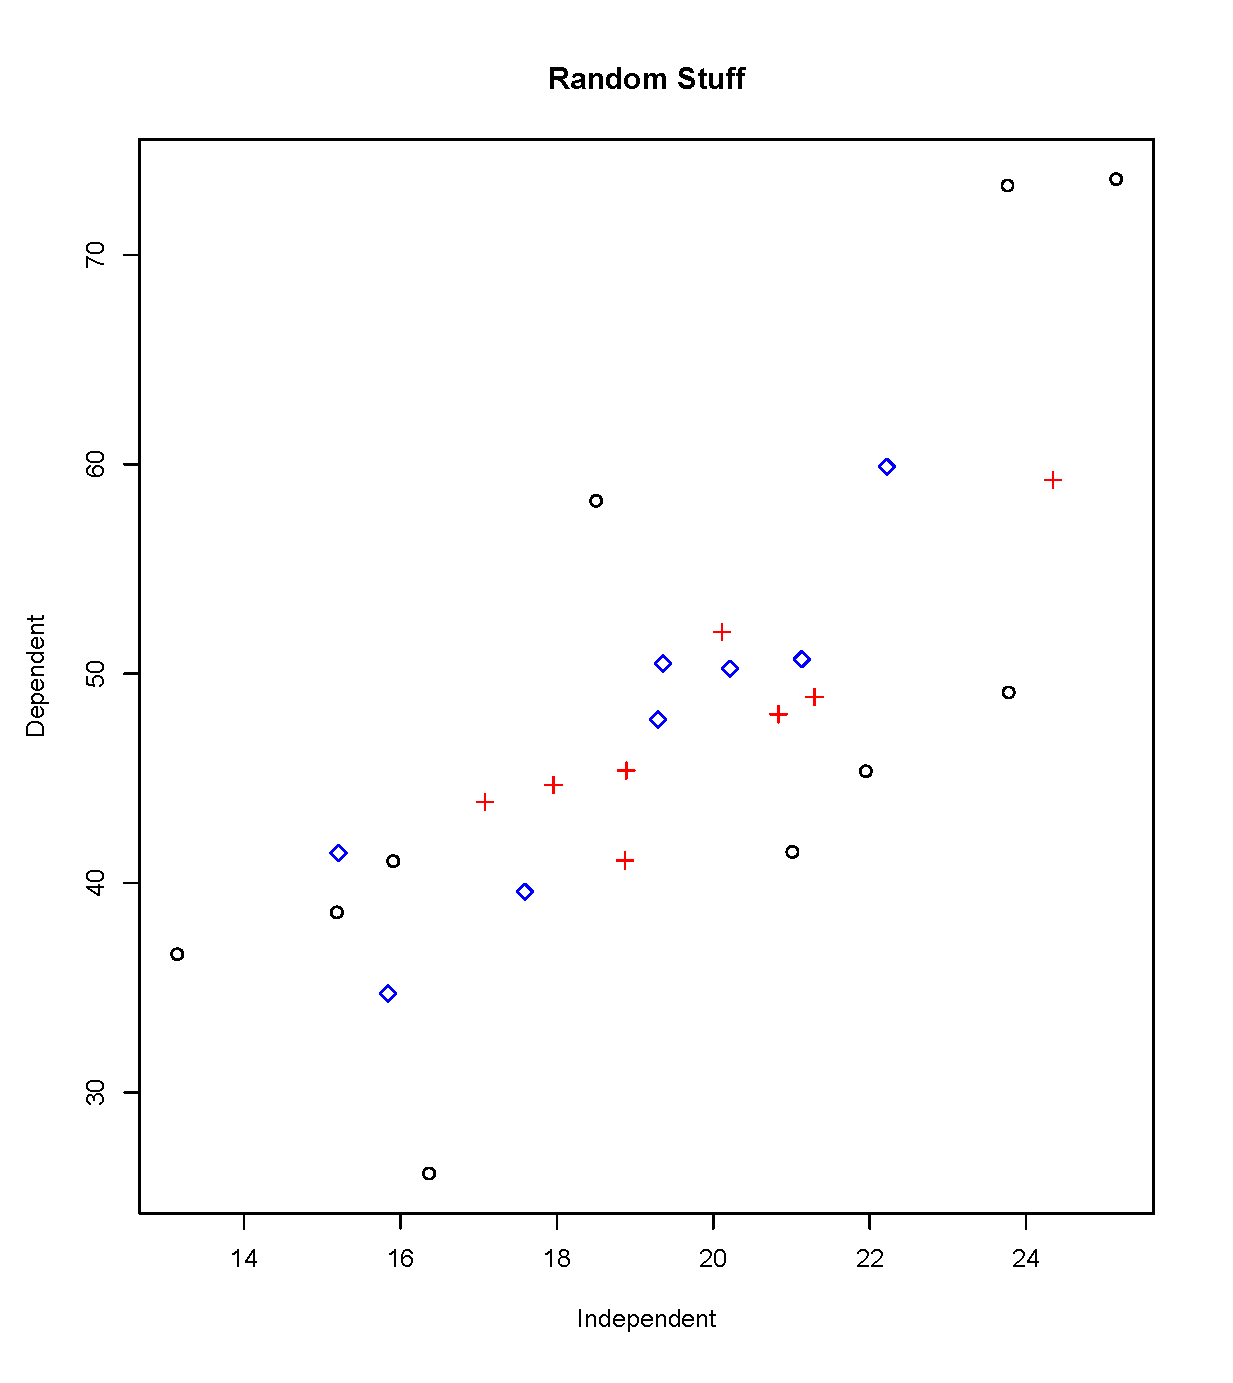
\includegraphics[width=\maxwidth]{knitr-cache/unnamed-chunk-3-1} 

\end{knitrout}
\end{center}
%\vspace{0mm}
\caption{Random points example... Degrees are represented in \latex like this 0.1$^\circ$ and superscript like this km$^2$)}
\label{fig:example-random-stuff}
\end{figure}
%%%%%%%%%%%%%%%%%%%%%%%
\clearpage


%%\begin{figure}[!htp]
%%\begin{center}
%%\includegraphics[width=6in,keepaspectratio=true]{maindoc/ARFMaturity.png}
%%\end{center}
%\vspace{0mm}
% To get the grid size in km^2 for the caption:
% While in the gui for the map, type mean(xtcall(PBSmap)$pdata$area) for the map you currently have loaded.
%\caption{Mean catch-per-unit-effort (CPUE, kg/h) of \fishname\ in grid cells 0.1$^\circ$ longitude by 0.075$^\circ$ latitude (roughly 57.8~km$^2$). The shaded cells give an approximation of the area where \fishname\ was encountered by fishing events from the groundfish trawl fishery from January 1, 1996 to October 7, 2014. Contours are 200 m and 1000 m isobaths. Red lines are PFMA area boundaries.} \label{fig:cpue} \end{figure}
%%\caption{Mean Maturity} \label{fig:maturity} \end{figure}
%%%%%%%%%%%%%%%%%%%%%%%

\begin{figure}[H]
\begin{center}
\begin{knitrout}
\definecolor{shadecolor}{rgb}{0.969, 0.969, 0.969}\color{fgcolor}
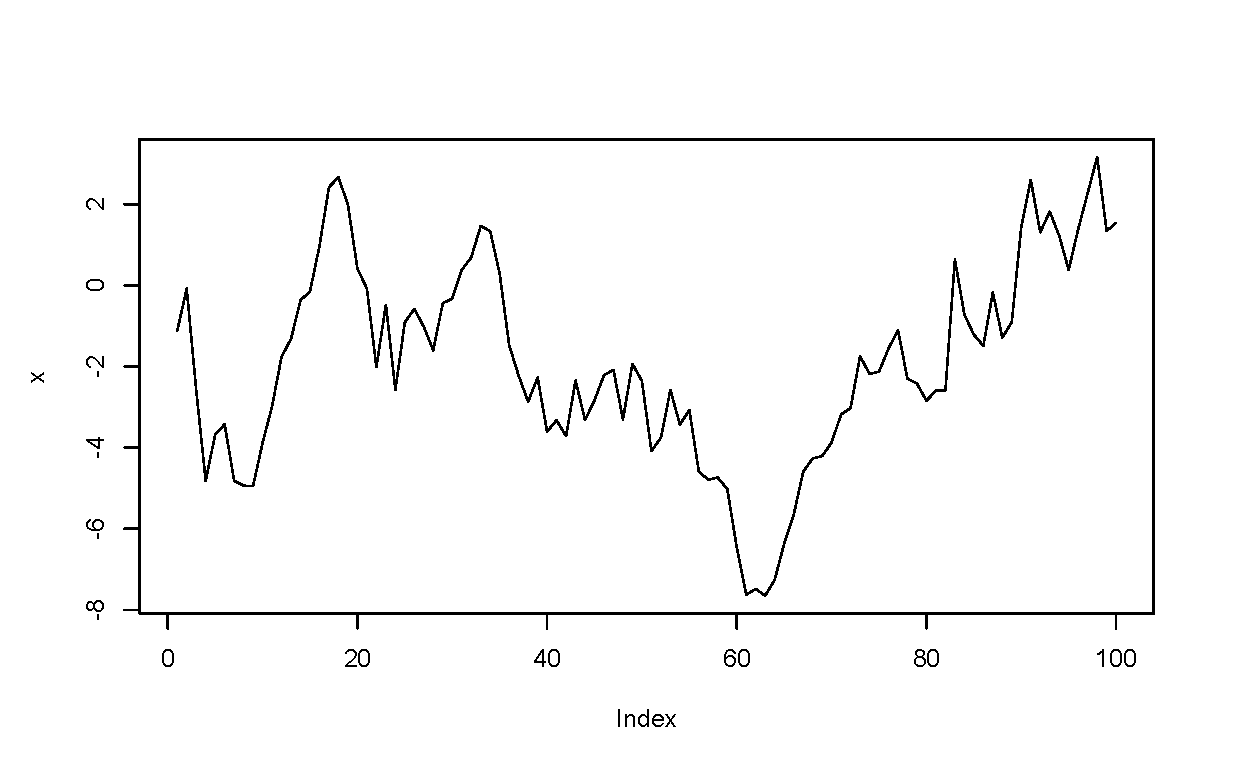
\includegraphics[width=\maxwidth]{knitr-cache/unnamed-chunk-4-1} 

\end{knitrout}
\end{center}
%\vspace{0mm}
\caption{Brownian motion example..}
\label{fig:example-brownian-motion}
\end{figure}
%%%%%%%%%%%%%%%%%%%%%%%

%%%%%%%%%%%%%%%%%%%%%%%
\begin{figure}[H]
\begin{center}
\begin{knitrout}
\definecolor{shadecolor}{rgb}{0.969, 0.969, 0.969}\color{fgcolor}
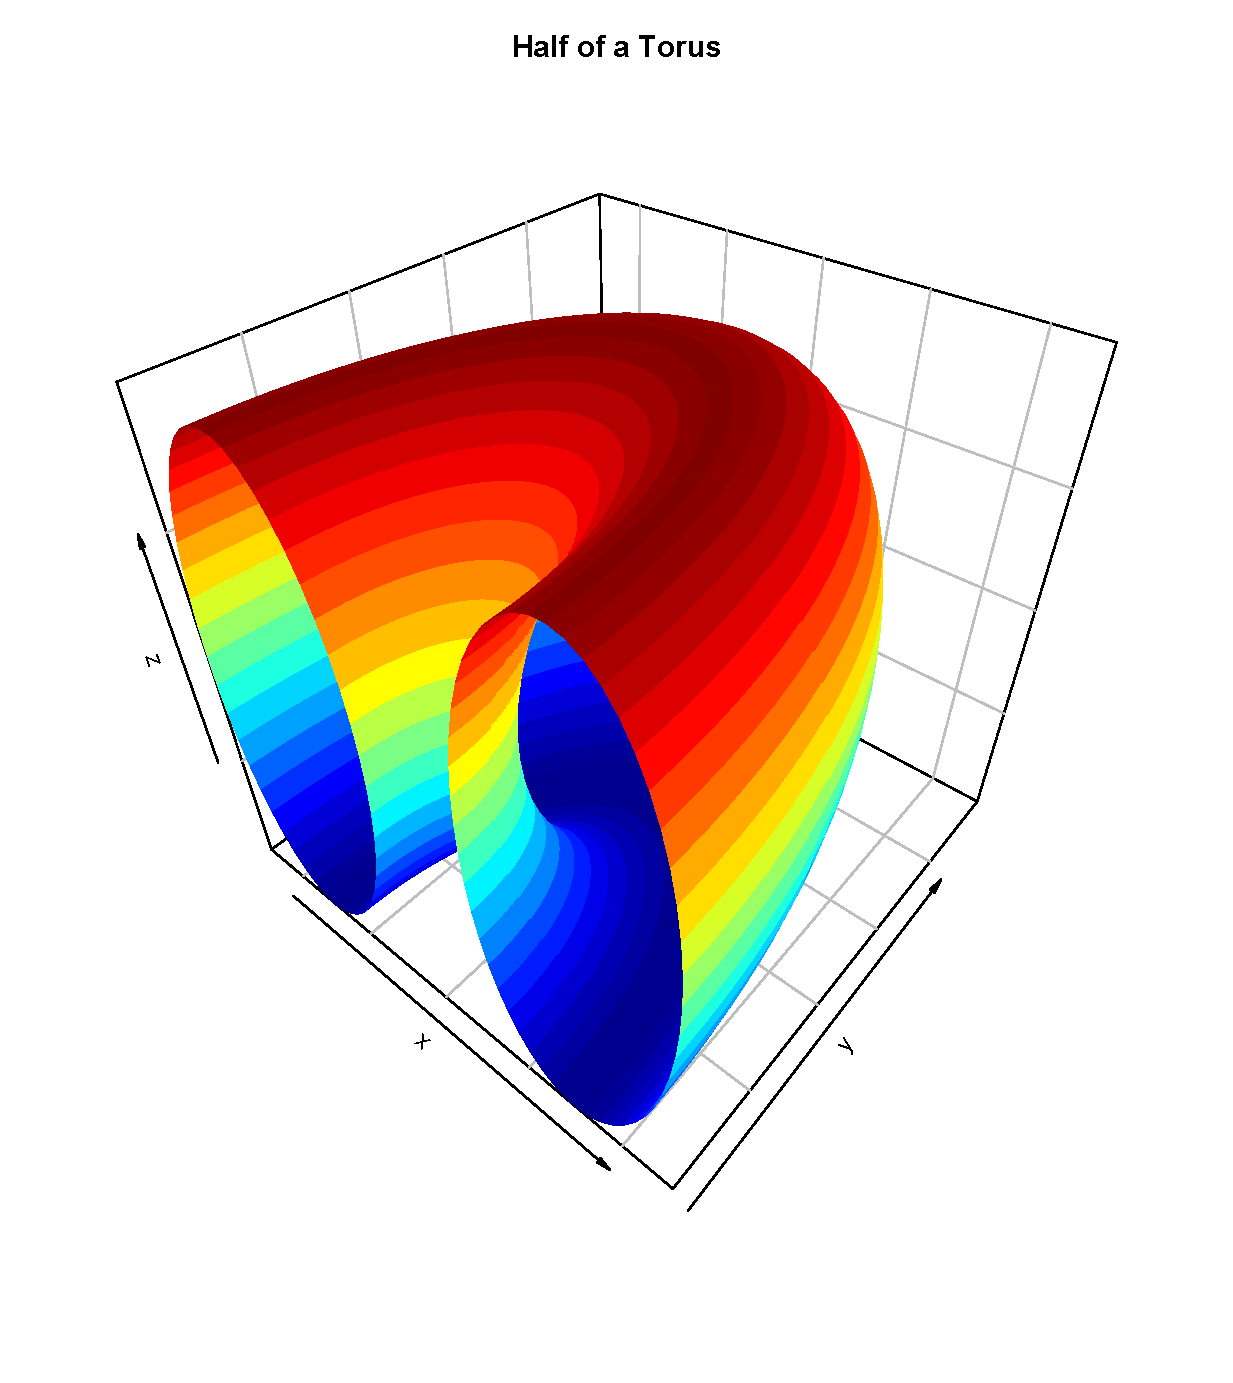
\includegraphics[width=\maxwidth]{knitr-cache/unnamed-chunk-5-1} 

\end{knitrout}
\end{center}
%\vspace{0mm}
\caption{Half torus example..}
\label{fig:example-half-torus}
\end{figure}
%%%%%%%%%%%%%%%%%%%%%%%
\clearpage

%%%%%%%%%%%%%%%%%%%%%%%
\begin{figure}[H]
\begin{center}
\begin{knitrout}
\definecolor{shadecolor}{rgb}{0.969, 0.969, 0.969}\color{fgcolor}
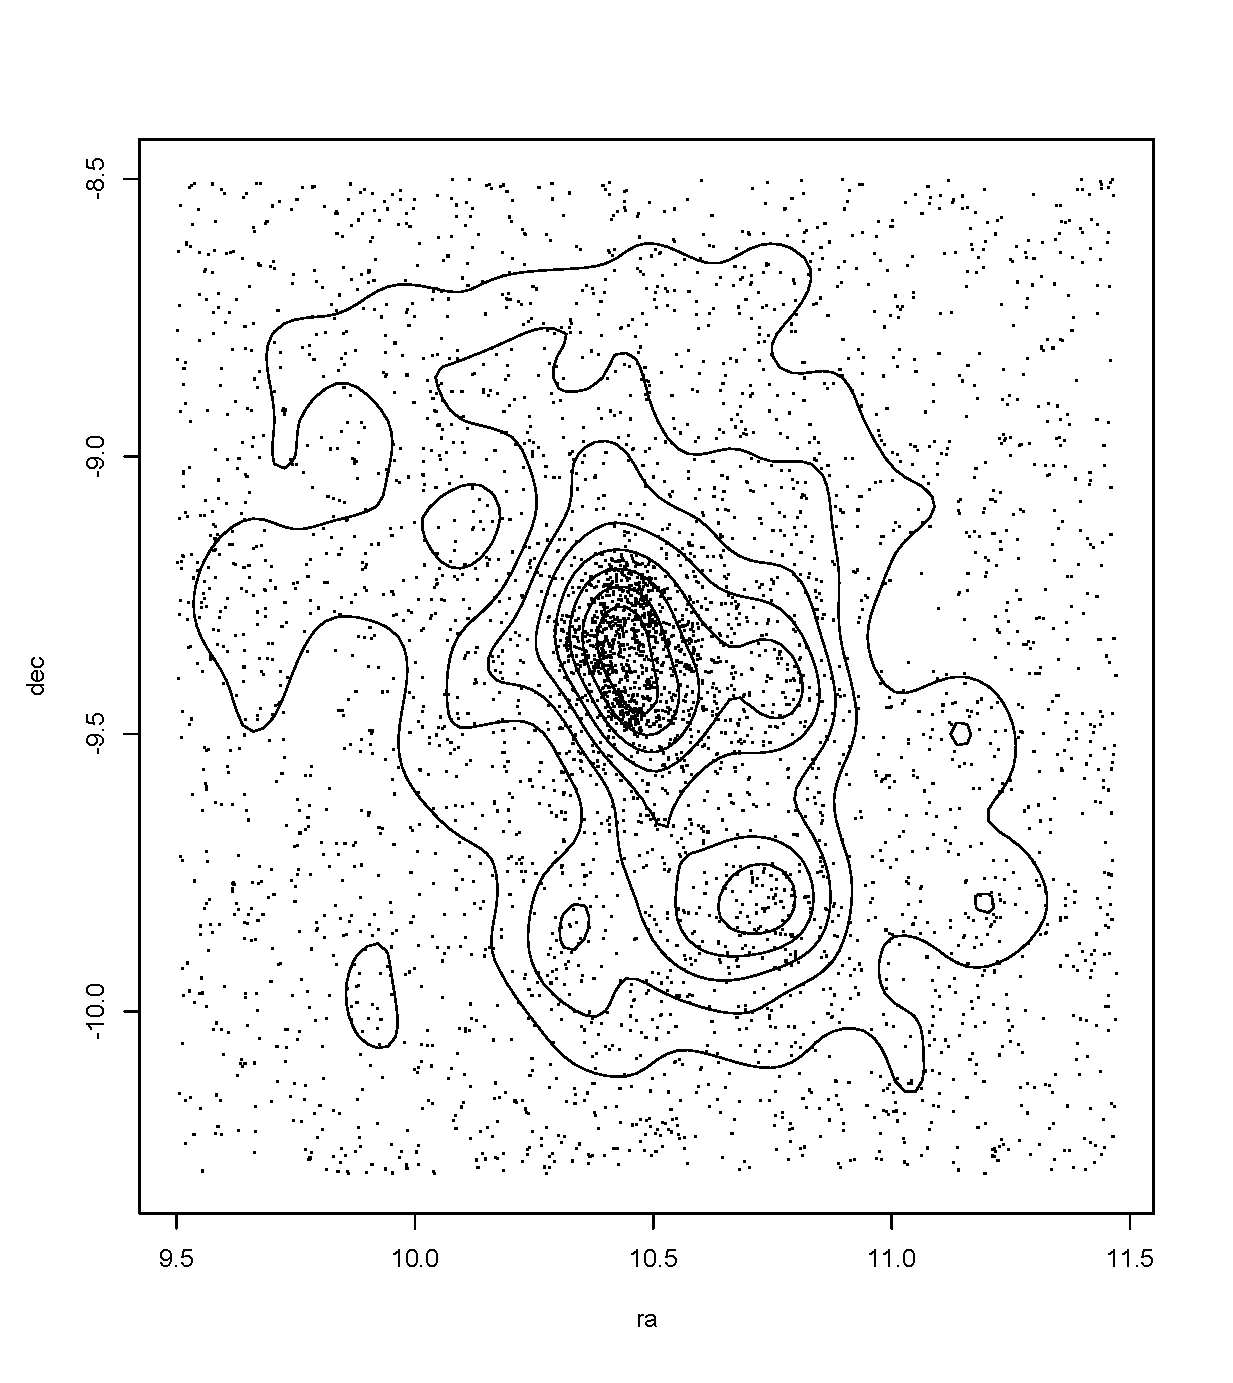
\includegraphics[width=\maxwidth]{knitr-cache/unnamed-chunk-6-1} 

\end{knitrout}
\end{center}
%\vspace{0mm}
\caption{Galaxy example}
\label{fig:example-galaxy}
\end{figure}
%%%%%%%%%%%%%%%%%%%%%%%

\clearpage

\addtocontents{toc}{\par {\bf \vspace{10mm} APPENDICES} \par}
\addtocontents{toc}{\protect\setcounter{tocdepth}{0}}
\appendix

%% Now want to number sections, tables etc. as A.1, A.2, etc.
%% Thought these wouldn't be with the appendix package, as
%%  automatic, but do need them even if use \begin{appendices}:
\renewcommand{\thesection}{\thechapter.\arabic{section}}
\renewcommand{\thetable}{\thechapter.\arabic{table}}
\renewcommand{\thefigure}{\thechapter.\arabic{figure}}
\renewcommand{\theequation}{\thechapter.\arabic{equation}}

%% Not including Appendix figures and tables in contents, and just
%%  including the Appendix (chapter) names (not sections or
%%  subsections):

\lfoot{Example \latex-knitr}

%% Add an appendix. The appedices or any other Rnw files will be in the same scope as the main file,
%% so they see the same R objects and those objects can be referenced directly.
%% There is no difference between this and maindoc, they are both pasted in directly
%% before the code is knitted.
\rfoot{Appendix A -- Example appendix 1}

% appendix-1.Rnw

% Some macros for equations found in tables
\def\beq{\vspace{-5ex} \begin{fleqn} \begin{equation}}
\def\eeq{\end{equation} \end{fleqn} \vspace{-5ex}}
\def\tabline{\vspace{2ex} \hrule \vspace{2ex}}
% new page macro
\def\newp{\vfill \break}

\clearpage

\chapter{Example appendix 1}
\label{chap:example.1}

\section{INTRODUCTION}

Stock Assessment modelling was done using the Integrated Statistical Catch Age Model (iSCAM), developed by S. Martell (\citet{martell2011}). iSCAM is written in AD Model Builder and the source code and documentation for the original iSCAM is available at \hyperref[https://github.com/smartell/iSCAM]{\color{blue}https://github.com/smartell/iSCAM}. Code for the version used in this assessment can be found at \hyperref[https://github.com/cgrandin/iSCAM]{\color{blue}https://github.com/cgrandin/iSCAM}. iSCAM uses a statistical catch-at-age model implemented in a Bayesian estimation framework.

Running of iSCAM and compilation of results figures was streamlined using the iscam-gui software package developed at the Pacific Biological Station by C. Grandin (\hyperref[https://github.com/cgrandin/iscam-gui]{\color{blue}https://github.com/cgrandin/iscam-gui}). iscam-gui is written in the statistical language R, and provides a graphical user interface that allows users to run and show output of multiple iSCAM model scenarios in a comparative fashion.

\section{MODEL DESCRIPTION}

Note we can reference tables in the main document by using the ref keyword. Here we reference the table with random numbers in it: Table \ref{tab:example-xtable}. Note that this reference \emph{tab:example-table} was given to the R function make.xtable as an argument. See maindoc.Rnw.

We can also reference any equation found anywhere, such as \ref{eq:sweptareaindex} which is referenced by the tag \emph{eq:sweptareaindex} or \ref{eq:cpuecalc} which is referenced by \emph{eq:cpuecalc}.

\section{ANALYTIC METHODS: EQUILIBRIUM CONSIDERATIONS}

\subsection{A Steady-State Age-Structured Model}

Here is another equation written in a slightly different way than in the maindoc. Latex allows for lots of different ways to do things:

\[s_o=\frac{\kappa}{\phi_E},\]
and the density-dependent term is given by:
\[\beta=\frac{\kappa-1}{R_{{o}}\phi_{{E}}}\]

Here is an example of an inline fraction: $s_o=\frac{\kappa}{\phi_E}$.

\section{RESIDUALS, LIKELIHOODS, AND OBJECTIVE FUNCTION VALUE COMPONENTS}
This is an example of nested lists using enumeration.. The objective function contains five major components:
\begin{enumerate}[noitemsep,nolistsep]
  \item The negative log-likelihood for the catch data
  \item The negative log-likelihood for the relative abundance data
  \item The negative log-likelihood for the age composition data
  \item The prior distributions for model parameters
  \item Three penalty functions that are invoked to regularize the solution during intermediate phases of the non-linear parameter estimation. The penalty functions:
  \begin{enumerate}[noitemsep,nolistsep]
    \item constrain the estimates of annual recruitment to conform to a Beverton-Holt stock-recruit function
    \item weakly constrain the log recruitment deviations to a normal distribution
    \item weakly constrain estimates of log fishing mortality to a normal distribution ($\sim N(\ln(0.2), 4.0)$) to prevent estimates of catch from exceeding estimated biomass.
    \end{enumerate}
\end{enumerate}


This example shows the use of some other special functions such as \emph{widehat} both inline and in equation form:
The residuals between the observed ($p_{t,a}$) and predicted proportions ($\widehat{p}_{t,a}$) is given by:
\begin{equation}\label{eq:widehat}
\eta_{t,a}=\ln(p_{t,a})-\ln(\widehat{p}_{t,a})-\frac{1}{A}\sum_{a=1}^A\left[\ln(p_{t,a})-\ln(\widehat{p}_{t,a}) \right]
\end{equation}
\clearpage

\newpage

\rfoot{Appendix B -- Example appendix 2}

\clearpage

\chapter{WEIGHTING OF AGE PROPORTIONS}
\label{chap:agecompweight}

This appendix summarizes a method for representing commercial and survey age structures for a given species through weighting observed age frequencies~$x_a$ or proportions~$x^\prime_a$ by \eor{catch}{density} in defined strata. The methodology presented in this appendix is based on that presented by \citet{rocksole2014} for Rock Sole.\\
\bigskip

Ideally, sampling effort would be proportional to the amount of the species caught, but this is not usually the case. Therefore, the stratified weighting scheme presented below attempts to adjust for unequal sampling effort among strata. For commercial samples, strata comprise quarterly periods within a year, while for survey samples, the strata are defined by longitude, latitude, and depth. Within each stratum, commercial ages are weighted by the catch weight (kg) of the species in tows that were sampled, and survey ages are weighted by the catch density (kg/km$^2$) of the species in sampled tows. A second weighting is then applied: quarterly commercial ages are weighted by the commercial catch weight of the species from all tows within each quarter; stratum survey ages are weighted by stratum areas (km$^2$) in the survey. Throughout this section, we use the symbol \sQuote{$\Vert$} to delimit parallel values for commercial and survey analyses, respectively, as the mechanics of the weighting procedure are similar for both. \\
\bigskip

For simplicity we illustrate the weighting of age frequencies $x_a$, unless otherwise specified. The weighting occurs at two levels: $h$ (quarters for commercial ages, strata for survey ages) and $i$ (years if commercial, surveys in series if survey). Notation is summarised in Table~\ref{tab:wtdAges}.\\
\bigskip

\usefont{\encodingdefault}{\familydefault}{\seriesdefault}{\shapedefault}\small
\begin{longtable}[1]{l>{\raggedright\arraybackslash}p{0.85\textwidth} }
%\caption{Equations for weighting age frequencies or proportions for \fishname.\\(\bold{c})~= commercial, (\bold{s})~= survey}
\caption{Equations for weighting age frequencies or proportions for Arrowtooth Flounder.\\(\textbf{c})~= commercial, (\textbf{s})~= survey}
\label{tab:wtdAges} \\
\hline
Symbol & Description \\ %\tstrut \bstrut \\
\hline
%& \tstrut \textbf{Indices} \bstrut \\
& \textbf{Indices} \\
$\bM{a}$ & age class (1 to $A$, where $A$ is an accumulator age-class) \\
$\bM{d}$ & (\textbf{c}) trip IDs as sample units \\
& (\textbf{s}) sample IDs as sample units \\
$\bM{h}$ & (\textbf{c}) quarters (1 to 4), 91.5 days each \\
& (\textbf{s}) strata (area-depth combinations) \\
$\bM{i}$ & (\textbf{c}) calendar years (1977 to present) \\
& (\textbf{s}) survey IDs in survey series (e.g., QCS Synoptic) \\ %\bstrut \\
\hline
%& \tstrut \textbf{Data} \bstrut \\
& \textbf{Data} \\
$\bM{x_{adhi}}$ & observations-at-age $a$ for sample unit $d$ in \eor{quarter}{stratum} $h$ of \eor{year}{survey} $i$ \\
$\bM{x^\prime_{adhi}}$ & proportion-at-age $a$ for sample unit $d$ in \eor{quarter}{stratum} $h$ of \eor{year}{survey} $i$ \\
$\bM{C_{dhi}}$ & (\textbf{c}) commercial catch (kg) of a given species for sample unit $d$ in quarter $h$ of year $i$ \\
& (\textbf{s}) density (kg/km$^2$) of a given species for sample unit $d$ in stratum $h$ of survey $i$ \\
$\bM{C^\prime_{dhi}}$ & $C_{dhi}$ as a proportion of total \eor{catch}{density} $C_{hi} = \sum_{d} C_{dhi}$ \\
$\bM{y_{ahi}}$ & weighted age frequencies at age $a$ in \eor{quarter}{stratum} $h$ of \eor{year}{survey} $i$ \\
$\bM{K_{hi}}$ & (\textbf{c}) total commercial catch (kg) of species in quarter $h$ of year $i$ \\
& (\textbf{s}) stratum area (km$^2$) of stratum $h$ in survey $i$ \\
$\bM{K_{hi}^\prime}$ & $K_{hi}$ as a proportion of total \eor{catch}{area} $K_i = \sum_{h} K_{hi}$ \\
$\bM{p_{ai}}$ & weighted frequencies at age $a$ in \eor{year}{survey} $i$ \\
$\bM{p_{ai}^\prime}$ & weighted proportions at age $a$ in \eor{year}{survey} $i$ \\ %\bstrut \\
\hline 
% \end{tabular}
% \end{center}
\end{longtable}
\usefont{\encodingdefault}{\familydefault}{\seriesdefault}{\shapedefault}\normalsize

For each \eor{quarter}{stratum} $h$ we weight sample unit frequencies $x_{ad}$ by sample unit \eor{catch}{density} of the assessment species. For commercial ages, we use trip as the sample unit, though at times one trip may contain multiple samples. In these instances, multiple samples from a single trip will be merged into a single sample unit. Within any \eor{quarter}{stratum} $h$ and \eor{year}{survey} $i$ there is a set of sample \eor{catches}{densities} $C_{dhi}$ that can be transformed into a set of proportions:
%
\eqn{C_{dhi}^\prime = \gfrac{C_{dhi}}{\sum_{d} C_{dhi}}~.}
%
The proportion $C_{dhi}^\prime$ is used to weight the age frequencies $x_{adhi}$ summed over $d$, which yields weighted age frequencies by \eor{quarter}{stratum} for each \eor{year}{survey}:
%
\eqn{y_{ahi} = \sum_{d} \big(C_{dhi}^\prime x_{adhi}\big)~.}
%
This transformation reduces the frequencies $x$ from the originals, and so we rescale (multiply) $y_{ahi}$ by the factor
%
\eqn{\gfrac{\sum_{a} x_{ahi}}{\sum_{a} y_{ahi}}}
%
to retain the original number of observations.

At the second level of stratification by \eor{year}{survey} $i$, we calculate the the annual proportion of quarterly catch (t) for commercial ages or the survey proportion of stratum areas (km$^2$) for survey ages
%
\eqn{K_{hi}^\prime = \gfrac{K_{hi}}{\sum_{h} K_{hi}}}
%
to weight $y_{ahi}$ and derive weighted age frequencies by \eor{year}{survey}:
%
\eqn{p_{ai} = \sum_{h} \big(K_{hi}^\prime y_{ahi}\big)~.}
%
Again, if this transformation is applied to frequencies, it reduces them from the original, and so we rescale (multiply) $p_{ai}$ by the factor
%
\eqn{\gfrac{\sum_{a} y_{ai}}{\sum_{a} p_{ai}}~.}
%
to retain the original number of observations.

Finally, we standardise the weighted frequencies to represent proportions-at-age:
%
\eqn{p_{ai}^\prime = \gfrac{p_{ai}}{\sum_{a} p_{ai}}~.}
%
If initially we had used proportions $x_{adhi}^\prime$ instead of frequencies $x_{adhi}$ , the final standardisation would not be necessary. However, its application does not affect the outcome.\\
\bigskip

The choice of data input (frequencies $x$ \emph{vs}. proportions $x^\prime$) can sometimes matter: the numeric outcome can be very different, especially if the input samples comprise few observations. Theoretically, weighting frequencies emphasises our belief in individual observations at specific ages while weighting proportions emphasises our belief in sampled age distributions. Neither method yields inherently better results. However, if the original sampling methodology favoured sampling few fish from many tows rather than sampling many fish from few tows, then weighting frequencies probably makes more sense than weighting proportions. In this assessment, we weight age frequencies $x$.

\newpage

%% Used when you need to insert outside documents:
%% \setcounter{page}{68}

\end{document}
